\section{Models}
\label{sec:models}

\subsection{Challenges and Modalities}
The previous section has yielded interesting results from human labelling (Section \ref{sec:human}). We concluded that a temporal dimension, and a lexical compensator might help in improving existing FER models for speaking subjects. 

Our current FER models are all working on static images, which means that we will have to temporalize them in some way. We will discuss this in section \ref{sub:temp}. A lexical compensator will have to be done with a separate model. There are many different approaches to this. We will discuss this in section \ref{sub:lex}.


\subsection{Temporal Dimension}
\label{sub:temp}
As discussed previously, we want to keep and build on existing FER models. Given that some of our models will work on video data, we will have to temporalize our models which currently work on static images.

The straight forward approach is to take the current model, and wrap it in a temporal layer. This means that an input video with 60 frames will produce 60 output embeddings, which can then be fed into a recurrent layer like a LSTM or GRU. This produces minimal overhead, while preserving all weights from our model.

We will use this approach in all our upcoming models.

\begin{figure}
    \centering
    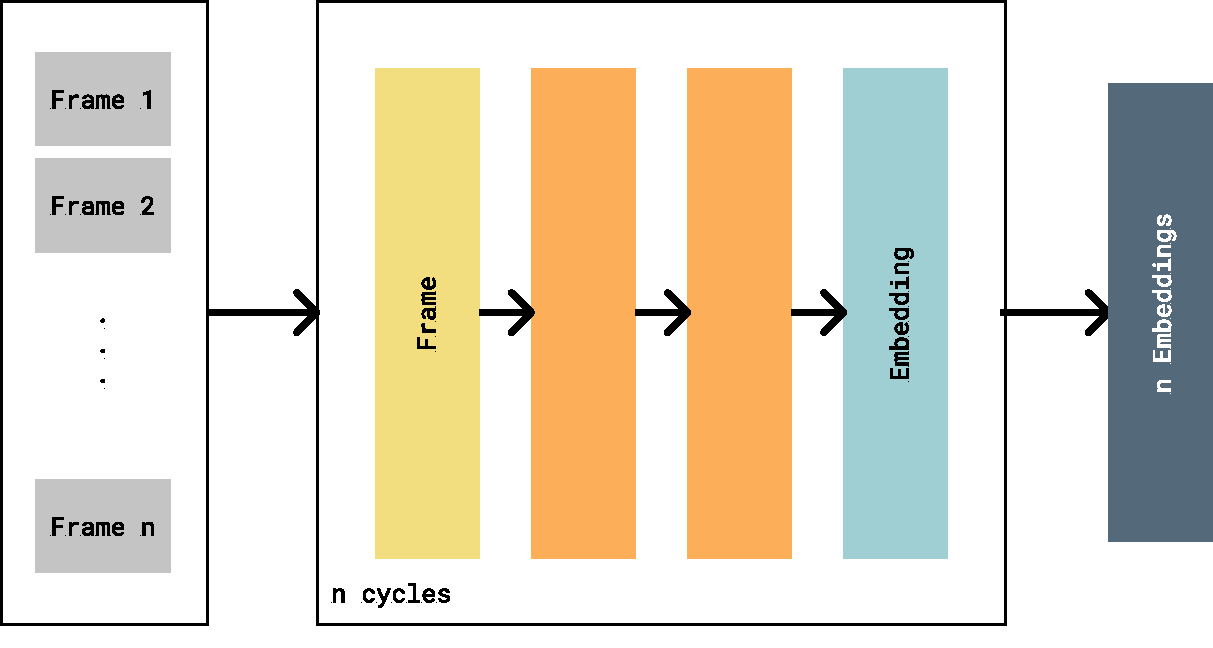
\includegraphics[width=0.8\textwidth]{res/temporalization.pdf}
    \caption{Temporalizing an FER model. The existing model gets wrapped in a TimeDimensional layer. That way the model produces $n$ embeddings for $n$ inputs.}
    \label{fig:temporalization}
\end{figure}

\subsection{Lexical Compensators}
\label{sub:lex}